\chapter{Характеристические функции. Предельные теоремы}
\setcounter{equation}{0}
\section{Производящие функции. Факториальные моменты}
Пусть задана дискретная целочисленная неотрицательная случайная величина $\xi$, $m = 0, 1, 2, \ldots$ – возможные значения. Закон распределения, которому подчиняется $\xi$: 
\[
	\Prob \{ \xi = m \} = p_m, \sum\limits_{m = 0}^{\infty} p_m = 1
\]
Такой закон удобно исследовать с помощью производящих функций. Пусть $u \in \mathbb{R}^1$. Определим производящую функцию дискретной случайной величины
\begin{equation}
	\Psi_{\xi} (u) \underset{\textrm{def} }{=} \MExpect_{u^{\xi}} = \sum\limits_{m} p_m \cdot u^m, \ |u| \leqslant 1
\end{equation}
Рассмотрим данный ряд. Он абсолютно сходится для $|u| \leqslant 1$
\begin{equation}
	p_m = \frac{1}{m!} \left. \frac{d^m \psi_{\xi} (u)}{du^{m}} \right|_{u = 0}
\end{equation}
\[
	\xi : \{ p_k \}, \psi_{\xi} (u), \psi_{\xi}(1) = 1
\]
Существует взаимно однозначное соответствие между производящими функциями и соответствующими законами распределения
\begin{theorem}
	Пусть задан набор целочисленных неотрицательных независимых случайных величин $\xi_1, \ldots, \xi_n$. Обозначим $\xi_k \sim \psi_{\xi_k} (u)$, то есть каждому элементу соответствует производящая функция. Тогда
\[
	\psi_{\xi_1 + \ldots + \xi_n} (u) = \prod\limits_{k = 1}^{n} \psi_{\xi_k} (u)
\]
\end{theorem}
\begin{proof}
	$u^{\xi_1}, \ldots, u^{\xi_n}$ --- независимы, поскольку $\xi_1, \ldots, \xi_n$ независимы. $g(x) = a^x$
\[
	\MExpect_{u^{\xi_1 + \ldots + \xi_n}} = \MExpect_{u^{\xi_1} \cdot \ldots \cdot u^{\xi_n}} = \prod\limits_{k = 1}^{n} \MExpect_{u^{\xi_k}}
\]
\end{proof}
\begin{example}
	Рассмотрим закон распределения Бернулли $B[n, p]$. $\xi_i$ --- число появления успеха в $i$-ом испытании.
\[
	\mu_n = \sum\limits_{i = 1}^{n} \xi_i, \ \psi_{\mu_n} (u) = \prod\limits_{k = 1}^{n} \psi_{\xi_k} (u)
\]
\[
	\psi_{\xi_k} (u) = \MExpect_{u^{\xi_k}} = u^0 q + u^1 p, \ \psi_{\mu_n} (u) = (pu + q)^n
\]
\[
	\Prob \{ \xi + \eta = n \} = \sum\limits_{k = 0}^{n} \Prob \{ \xi = k \} \cdot \Prob \{ \eta = n - k \}
\]
Используя теорему 1, можно найти композицию (свёртку) распределения, не прибегая к формуле свёртки.
\end{example}
\begin{theorem}
	Пусть задан набор целочисленных неотрицательных независимых одинаково распределённых случайных величин $\xi_1, \ldots, \xi_n$
\[
	\forall k: \xi_k \sim \psi_{\xi} (u)
\]
\[
	\left.
	\begin{aligned}
	\eta_{\nu} = \xi_1 + \ldots + \xi_{\nu}, \nu \geqslant 1 \\
	\eta_{\nu} = 0, \nu < 1
	\end{aligned}
	\right	\} \Rightarrow \psi_{\eta_{\nu}} (u) = \psi_{\nu} (\psi_{\xi} (u))
\]
\end{theorem}
\begin{proof}
\[
	\MExpect [u^{\xi_1 + \ldots + \xi_{\nu}} \ | \ \nu = n] = \MExpect_{u^{\xi_1 + \ldots + \xi_n}} = \left[ \psi_{\xi} (u) \right]^n
\]
$n \in \mathbb{N}$
\[
	\psi_{\eta_{\nu}} (u) \overset{\textrm{def}}{=} \MExpect_{u^{\eta_{\nu}}} = \MExpect \left[ \MExpect \left[ u^{\eta_{\nu}} \ | \ \nu \right] \right] = \MExpect \left[ \left[ \psi_{\xi} (u) \right]^{\nu} \right] = \psi_{\nu} \left( \psi_{\xi} (u)\right) 
\]
\end{proof}
\begin{definition}
	$k$-ым факториальным моментом целочисленной неотрицательной случайной величины $\xi$ называется математическое ожидание $\MExpect_{{\xi}^{[k]}}$, такое, что
    \[
	    \xi^{[k]} = \xi (\xi - 1) \ldots (\xi - k + 1)
    \] 
	\[
		m^{[k]} = m (m - 1) \ldots (m - k + 1)
	\]
	\[
		m^{[k]} = 0, \ m < k
	\]
	При $k = 0$: $\xi^{[0]} = 1$
	\[
		\MExpect_{\xi^{[1]}} = \MExpect_{\xi}, \ \MExpect_{\xi^{[2]}} = \MExpect_{\xi^{2}} - \MExpect_{\xi}
	\]
	\[
		\Variance_{\xi} = \MExpect_{\xi^{[2]}} + \MExpect_{\xi^{[1]}} - (\MExpect_{\xi^{[1]}})^2
	\]
\end{definition}
\begin{theorem}
	Если существует факториальный момент $k$-ого порядка $\MExpect_{\xi^{[k]}}$, то существует левосторонняя $k$-ая производная производящей функции
	\[
		\exists \MExpect_{\xi^{[k]}} \Rightarrow \exists \psi_{\xi}^{(k)} (1 - 0), \ \psi_{\xi}^{(k)} (1 - 0) = \MExpect_{\xi^{[k]}}
	\]
$|u| < 1$
\[
	\psi_{\xi}^{(k)} (u) = \sum\limits_{m = k}^{\infty} m^{[k]} \cdot u^{m - k} \Prob \{ \xi = m \}
\]
По второй теореме Абеля:
	\[
		\MExpect_{\xi^{[k]}} = \sum\limits_{m = k}^{\infty} m^{[k]} \Prob \{ \xi = m \}
	\]
\end{theorem}
\begin{theorem}
	\textit{(Абеля)} Пусть $r > 0$, тогда
	\[
		\sum\limits_{k = 0}^{\infty} a_k r^k = S
	\]
	\[
		\sum\limits_{k = 0}^{\infty} a_k x^k, x \in [0, r]
	\]
	\[
		\lim\limits_{x \to r - 0} \sum\limits_{k = 0}^{\infty} a_k x^k = S
	\]
\end{theorem}
Оказывается, что соответствие между рассмотренными законами распределения вероятностей и производящими функциями не только взаимно однозначно, но ещё и взаимно непрерывно.
\begin{theorem} \textit{(Непрерывность производящих функций)} 
	Пусть при фиксированном $n$ $(n = 1, 2, \ldots)$:
	\[
		{\{ p_k (n) \}}_{k = 0, 1, 2, \ldots} : p_k (n) \geqslant 0, \forall k
	\]
	\[
		\sum\limits_{k = 0}^{\infty} p_k (n) = 1
	\]
	\[
		\psi_m (u) = \sum\limits_{k = 0}^{\infty} p_k (n) u^k
	\]
	\[
		\lim\limits_{n \to \infty} p_k (n) = p_k, \ \sum\limits_{k = 0}^{\infty} p_k = 1 \Leftrightarrow \forall \; u:  0 < u \leqslant 1 \;\; \lim\limits_{n \to \infty} \psi_n (u) = \psi (u),
	\]
	где $\psi (u) = \sum\limits_{k = 0}^{\infty} p_k u^k$
\end{theorem}
\begin{example}
	Рассмотрим биномиальное распределение. $\mu_n, p_n$
	\[
		\lim\limits_{n \to \infty} \underbrace{n p_n}_{a_n} = a, \ \lim\limits_{n \to \infty} \Prob \{ \mu_n = m \}
	\]
	\[
		\psi_{\mu_n} (u) = \sum\limits_{m = 0}^{n} \Prob \{ \mu_n = m \} \cdot u^m = \left( \frac{a_n}{n} \cdot u + 1 - \frac{a_n}{n} \right)^n =
	\]
	\[
		= \left( 1 + \frac{a_n}{n} (u - 1) \right)^n \underset{n \to \infty}{\rightarrow} e^{a(u - 1)} = \sum\limits_{m = 0}^{\infty} \frac{a}{m!} e^{-a} u^m,
	\]
	То есть
	\[
		\Prob \{ \mu_n = m \} \underset{n \to \infty}{\rightarrow} \frac{a^m}{m!} e^{-a}
	\]
\end{example}
Рассмотрим случайный вектор $\overline{\xi} = (\xi_1, \ldots, \xi_n)$, где $\xi_i$ --- целочисленная непрерывная случайная величина. Также введём вектор значений $\overline{m} = (m_1, \ldots, m_n)$, не более чем счётный набор. То есть
\[
	\Prob_{\overline{m}} = \Prob \{ \overline{\xi} = \overline{m} \}
\]
Введём производящую функцию:
\[
	\psi_{\overline{\xi}} (u_1, \ldots, u_m) \overset{\textrm{def}}{=} \MExpect [u_1^{\xi_1} \cdot \ldots \cdot u_m^{\xi_m}] = \sum\limits_{\overline{m}} \Prob_{\overline{m}} \cdot u^{m_1} \cdot \ldots \cdot u^{m_n}
\]
Можем определить смешанный факториальный момент порядка $k_1 + \ldots + k_n, \ k_i \geqslant 0, \ i = 1, 2, \ldots n$
\[
	\MExpect_{\xi_1^{[k_1]} \cdot \ldots \cdot \xi_n^{[k_n]}}, \xi_i^{[k]} = \xi_i (\xi_i - 1) \ldots (\xi_i - k + 1), \ \xi^{[0]} = 1
\]
\[
	\MExpect_{\xi_1^{[k_1]} \cdot \ldots \cdot \xi_n^{[k_n]}} = 
\left. \frac{ \partial^{k_1 + \ldots + k_n} \psi_{\overline{\xi}} (u_1, \ldots, u_m) }{ \partial u_1^{k_1} \cdot \ldots \cdot \partial u_n^{k_n} } \right|_{u_1 = \ldots = u_n = 0}
\]

\section{Характеристические функции случайных величин}
Пусть $\xi$, $\eta$ --- случайные величины, $i: \ i^2 = -1$. Составим случайную величину $\theta = \xi + i \eta$. \\
Пусть также существуют математические ожидания введённых величин: $\MExpect_{\xi}$, $\MExpect_{\eta}$. Тогда можем составить математическое ожидание комплексно-значной случайной величины:
\[
	\MExpect_{\theta} = \MExpect_{\xi} + i \MExpect_{\eta} 
\]
Все свойства математического ожидания вещественно-значной случайной величины переносятся также на комплексно-значную случайную величину. \\
$\theta_1$ и $\theta_2$ независимы, если независимы два вектора $(\xi_1, \eta_1)$ и $(\xi_2, \eta_2)$.
\begin{definition}
	Характеристической функцией вещественно-значной случайной величины называется функция вещественного аргумента, которая представляет собой математическое ожидание $e^{it\xi}$:
\[
	\phi_{\xi} (t) = \MExpect_{e^{it\xi}}, \ t \in \mathbb{R}^1, \text{ $\xi$ --- вещественная случайная величина}
\]
\[
	e^{i \alpha} = cos \alpha + i sin \alpha
\]
\[
	\phi_{\xi} (t) = \MExpect [cos \xi t] + i \MExpect [sin \xi t]
\]
\[
	|e^{it\xi}| = 1, \ \theta = a + i b, \ |\theta| = \sqrt{a^2 + b^2}
\]
\[
	\phi_{\xi} (t) = \int\limits_{-\infty}^{+\infty} e^{itx} d \mathcal{P}_{\xi} (x)
\]
\end{definition}
Характеристическая функция полностью определяется распределением своей случайной величины. \\ \\
В случае, если $\xi$ --- абсолютно-непрерывная случайная величина
\[
	\phi_{\xi} (t) = \int\limits_{-\infty}^{+\infty} e^{itx} f_{\xi} (x) dx
\]
Если $\xi$ --- дискретная случайная величина:
\[
	\phi_{\xi} (t) = \sum\limits_{k} e^{itx_k} \cdot \Prob \{ \xi = x_k \},
\]
где $\{ x_k \}_{k = 1, \ldots}$ --- не более чем счётный набор
\subsection{Свойства характеристической функции случайной величины}
\begin{enumerate}[wide, labelwidth=!, labelindent=0pt]
	\item $|\phi(t)| \leqslant 1, \ \forall t \in \mathbb{R}^1, \ \phi(0) = 1$ \\
\[ | \MExpect_{e^{it \xi}} | \leqslant \MExpect_{|e^{it \xi}|} = 1 \]
	\item $\xi$ --- случайная величина, $a, b$ --- константы, $\eta = a \xi + b$
\[
	\phi_{\eta} (t) = \MExpect_{e^{it(a \xi + b)}} = e^{it b} \cdot \phi_{\xi} (at)
\]
$c$ --- константа
\[
	\phi_c (t) = e^{itc}
\]
	\item $\xi_1, \ldots, \xi_n$ --- независимые случайные величины. Тогда
\[
	\phi_{\xi_1 + \ldots + \xi_n} (t) = \prod\limits_{k = 1}^{n} \phi_{\xi_k} (t) \Rightarrow e^{it \xi_1}, \ldots, e^{it \xi_n} \text{ --- тоже независимые}
\]
\item $\phi_{\xi} (-t) = \phi_{- \xi} (t) = \overline{\phi_{\xi} (t)}$
\item $\xi \geqslant 0$, целочисленная случайная величина. Тогда производящая функция $\psi_{\xi} (u) = \MExpect_{u^{\xi}}$. Тогда
\[
	\phi_{\xi} (t) = \MExpect_{e^{it\xi}} = \psi_{\xi} (e^{it})
\]
\item Характеристическая функция равномерно непрерывна по аргументу $(t)$ на всей числовой оси
\[
	| \phi(t + h) - \phi(t) | = \Delta (h) \underset{h \to 0}{\rightarrow} 0, \ \forall t \in \mathbb{R}^1
\]
Покажем это.
\[
	\phi(t) = \int\limits_{-\infty}^{+\infty} e^{itx} d \mathcal{P}_{\xi} (x)
\]
\[
	| \phi (t + h) - \phi (t) | \leqslant \int\limits_{-\infty}^{+\infty} | e^{i (t + h) x} - e^{itx} | d \mathcal{P}_{\xi} (x) =
\]
Известно, что
\[
	| \theta_1 \cdot \theta_2 | = |\theta_1| \cdot | \theta_2 |, \ | e^{itx} | = 1
\]
\[
	= \int\limits_{-\infty}^{+\infty} \underbrace{| e^{ihx} - 1 |}_{g_h (x)} d \mathcal{P}_{\xi} (x) = \Delta (h) \underset{h \to 0}{\rightarrow} 0
\]
$g_h(x) \underset{h \to 0}{\rightarrow} 0$, $g_h(x) \leqslant 2, \forall x \in \mathbb{R}^1$
\subsection{Примеры}
\begin{itemize}
	\item $B [n, p]$, $q = 1 - p$
\[
	\phi_{\xi} (t) = (pe^{it} + q)^n
\]
	\item $\xi \sim P [a]$, $a > 0$, $e^{a(u - 1)}$
\[
	\phi_{\xi} (t) = exp \{ a(e^{it} - 1) \}
\]
    \item $\xi = c$ с вероятностью 1.
\[
	\phi_c (t) = e^{itc}
\] 
	\item $\xi \sim N(0, 1)$. Доказать самостоятельно:
\[
	\phi_{\xi} (t) = e^{- \frac{t^2}{2}}
\]
\item $\eta \sim N(a, \sigma)$, $a \in \mathbb{R}^1$, $\theta > 0$
\[
	\phi_{\eta} (t) = e^{{ita} - \frac{\sigma^2 t^2}{2}}
\]
\item $\xi \sim R [a, b]$
\[
	\phi_{\xi} (t) = \frac{e^{i t b} - e^{i t a}}{it(b - a)}
\]
\end{itemize}
\begin{theorem}
	\textit{(Формула обращения)} Пусть $\xi$ --- случайная величина, задана функция распределения $F(x)$, характеристическая функция $\phi(t)$. Пусть также $x_1 < x_2$ --- точки непрерывности $F(x)$. Тогда имеет место соотношение
\[
	F(x_2) - F(x_1) = \frac{1}{2 \pi} \cdot \lim\limits_{A \to + \infty} \int\limits_{-A}^{A} \frac{e^{-it x_1} - e^{-it x_2}}{it} \phi(t) dt
\]
\end{theorem}
\begin{proof}
\[
	\int\limits_{-\infty}^{+\infty} | \phi_{\xi} (t) | dt < \infty
\]
\[
	f_{\xi} (x) = \frac{1}{2 \pi} \int\limits_{-\infty}^{+\infty} e^{-it x} \cdot \phi(t) dt, \ a < b
\]
Проинтегрируем по $x$:
\[
	\int\limits_{a}^{b} f_{\xi} (x) dx = F(b) - F(a) = \int\limits_{a}^{b} \left[ \int\limits_{-\infty}^{+\infty} e^{-itx} \cdot \phi(t) dt \right] dx \overset{\text{т. Фубини}}{=}
\]
\[
	= \frac{1}{2 \pi} \int\limits_{-\infty}^{+\infty} \phi(t) \left[ \int\limits_{a}^{b} e^{-itx} dx \right] dt = \frac{1}{2 \pi} \int\limits_{-\infty}^{+\infty} \frac{e^{-ita} - e^{-itb}}{it} \phi(t) dt
\]
\end{proof}
\begin{theorem}
	Функция распределения однозначно определяется характеристической функцией своей случайной величины. 
\end{theorem}
Из предыдущей теоремы следует, что для любой точки непрерывности функции распределения соответствует формула обращения. Пусть $x$ --- точка непрерывности $F(x)$. Тогда
\[
	F(x) = \frac{1}{2 \pi} \lim\limits_{y \to -\infty} \lim\limits_{A \to +\infty} \int\limits_{-A}^{A} \frac{e^{-ity} - e^{-itx}}{it} \phi(t) dt
\]
\[
	F_{\xi} (x) = \lim\limits_{x_1 \downarrow x} F(x_1)
\]
\begin{example} 
	\begin{itemize}
		\item Пусть $\xi \sim N(a_1, \sigma_1)$, $\xi_2 \sim N(a_2, \sigma_2)$, где $\xi_1, \xi_2$ --- независимые случайные величины. Каков закон распределения $\xi_1 + \xi_2$?
\[
	\phi_{\xi_k} (t) = e^{it a_k - \frac{\sigma^2_k t^2}{2}}, \ k = 1, 2
\]
\[
	\phi_{\xi_1 + \xi_2} (t) = e^{it(a_1 + a_2) - \frac{(\sigma_1^2 + \sigma_2^2)t^2}{2}}
\]
\[
	\xi_1 + \xi_2 \sim N \left(a_1 + a_2, \sqrt{\sigma_1^2 + \sigma_2^2} \right)
\]
\item $\chi_n^2 = \xi_1^2 + \ldots + \xi_n^2$, $\xi_k \sim N (0, 1)$, $k = 1, \ldots, n$, $\xi_1, \ldots,\xi_n$ --- независимые случайные величины
	\end{itemize}
\end{example}
\begin{theorem}
	Пусть математическое ожидание $\MExpect_{|\xi|^n}$ некоторой случайной величины конечно. Тогда характеристическая функция $\xi$ дифференцируема $n$ раз и справедливо:
\[
	\phi_{\xi}^{(k)} (0) = i^k \MExpect_{\xi^k}, \ k \leqslant n
\]
\end{theorem}
Покажем это.
\[
	\phi_{\xi}^{(k)} (t) = i^k \int\limits_{-\infty}^{+\infty} e^{itx} \cdot x^k d \mathcal{P}_{\xi}
\]
\[
	\left| \int\limits_{-\infty}^{+\infty} x^k \cdot e^{itx} d \mathcal{P}_{\xi} \right| \leqslant \int\limits_{-\infty}^{+\infty} |x|^k d \mathcal{P}_{\xi} < \infty
\]
Рассмотрим логарифм характеристической функции
\[
	\kappa (t) = ln(\phi(t)), \ \kappa'(t) = \frac{\phi'(t)}{\phi(t)}
\]
\[
	\kappa''(t) = \frac{\phi''(t) \cdot \phi(t) - [\phi'(t)]^2}{[\phi(t)]^2}
\]
\[
	\kappa'(0) = \phi'(0) = i \cdot \MExpect_{\xi}
\]
\[
	\kappa''(0) = \phi''(0) - [\phi'(0)] = - \Variance_{\xi}
\]
\begin{definition}
	Производная $k$-ого порядка логарифма характеристической функции случайной величины $\xi$ в нуле, умноженная на $i^k$, называется семиинвариантом $k$-ого порядка случайной величины $\xi$
\end{definition}
Семиинвариант суммы независимых случайных величин равен сумме семиинвариантов слагаемых того же порядка. \\
Семиинвариант любого порядка есть рациональная функция моментов порядков не превосходящих $k$. \\
При сложении независимых случайных величин их функции распределения свёртываются, характеристические перемножаются, семиинварианты складываются.

\item Пусть математическое ожидание некоторой случайной величины $\xi$ конечно $\MExpect_{|\xi|^n}$. Тогда имеет место:
\[
	\phi(t) = \sum\limits_{k = 0}^{n} \frac{(it)^k}{k!} \MExpect_{\xi}^k + o(|t|^n)
\]
\[
	\phi(t) = \phi(0) + t \cdot \phi'(0) + \frac{t^2}{2} \phi''(0) + o(t^2) = 
\]
\[
	= 1 + it \cdot \MExpect_{\xi} - \frac{t^2}{2} \MExpect_{\xi^2} + o(t^2)
\]

\begin{theorem}
	\[
		\forall x: \ F_n (x) \underset{n \to \infty}{\rightarrow} F(x) \Leftrightarrow \phi_n (t) \underset{n \to \infty}{\rightarrow} \phi(t)
	\]
где $x$ --- точка непрерывности $F(x)$. \\
Чтобы последовательность функций распределения $F_n$ сходилась в каждой точке к предыдущей функции распределения, необходимо и достаточно, чтобы последовательность соответствующих характеристических функций в каждой точке $t$ сходилась к характеристической функции, соответствующей этой функции распределения. \\
Если $\phi$ --- вещественная, то она чётная.
\end{theorem}
\end{enumerate}
\begin{definition}
	Пусть имеется $\overline{\xi} = (\xi_1, \ldots, \xi_n)$, $F_{\xi} (x_1, \ldots, x_n) = \Prob(\xi_1 \leqslant x_1, \ldots, \xi_n \leqslant x_n)$. Характеристической функцией случайного $n$-мерного вектора будем называть $n$-мерную функцию, которая представляет собой:
\[
	\phi_{\overline{\xi}} (\overline{t}) = \MExpect_{e^{i(\overline{t}, \overline{\xi})}}, \ (\overline{t}, \overline{\xi}) = \sum\limits_{k = 1}^{n} t_k \xi_k
\]
где $\overline{t} = (t_1, \ldots, t_n) \in \mathbb{R}^n$
\[
	\phi_{\xi} (\overline{t}) = \int\limits_{\mathbb{R}^n} e^{i(\overline{t}, \overline{x})} d F_{\overline{\xi}} (\overline{x})
\]
\end{definition}
\subsection{Свойства характеристической функции случайного вектора}
\begin{enumerate}
	\item $\forall \overline{t} \in \mathbb{R}^n$, $|\phi_{\overline{\xi}} (\overline{t}) | \leqslant 1$, $\phi (\overline{0}) = 1$
	\item $\phi(\overline{t})$ равномерно непрерывна по $\overline{t} \in \mathbb{R}^n$
	\item Пусть $m < k$, тогда
\[
	\phi_{\xi_1, \ldots, \xi_m} (t_1, \ldots, t_m) = \phi_{\xi_1, \ldots, \xi_k} (t_1, \ldots, t_m, 0, \ldots, 0)
\]
	\item Пусть 
	\[
		\phi_{\xi_1 + \ldots + \xi_n} (t) = \phi_{\xi_1, \ldots, \xi_n} \underbrace{(t, t, \ldots, t)}_{n}, \ t \in \mathbb{R}^1
	\]
	Тогда
	\[
		\sum\limits_{k = 1}^{n} t \xi_k = t \sum\limits_{k = 1}^{n} \xi_k
	\]
	\item $\overline{\eta} = C \overline{\xi} + \overline{b}$
	\[
		\phi_{\overline{\eta}} (\overline{t}) = e^{i(\overline{t}, \overline{b})} \cdot \phi_{\overline{\xi}} (C^T \overline{t})
	\]
	\item $\phi_{\overline{\xi}} (- \overline{t}) = \overline{\phi_{\overline{\xi}}(\overline{t})} = \phi_{- \overline{\xi}} (\overline{t})$
	\item Можем рассмотреть смешанные моменты, $k_m \geqslant 0$, $m = 1, \ldots, n$:
	\[
		\MExpect [\xi_1^{k_1} \cdot \ldots \cdot \xi_n^{k_n}] = \left. i^{-K} \frac{\partial^K \phi_{\overline{\xi}} (t_1, \ldots, t_n)}{\partial t_1^{k_1} \ldots \partial t_n^{k_n}} \right|_{t_1 = \ldots = t_n = 0}
	\]
	\[
		\sum\limits_{m = 1}^{n} k_m = K > 0
	\]
	\item $\xi_i \geqslant 0$, целочисленные случайные величины, $i = 1, \ldots, n$
	\[
		\Psi_{\overline{\xi}} (u_1, \ldots, u_n) = \MExpect_{u_1^{\xi_1} \ldots u_n^{\xi_n}}
	\]
	Выразим характеристическую функцию через производящую:
	\[
		\phi_{\overline{\xi}} (t_1, \ldots, t_n) = \Psi_{\overline{\xi}} (e^{it_1}, \ldots, e^{it_n})
	\]
\end{enumerate}
\begin{example}
	\begin{enumerate}
		\item Полиномиальное распределение 
		\[
			\Psi_{\overline{\xi}} (u_1, \ldots, u_n) = (p_1 u_1 + \ldots + p_n u_n)^m
		\]
		\[
			\phi_{\overline{\xi}} (t_1, \ldots, t_n) = (p_1 e^{it_1} + \ldots + p_n e^{it_n})^m
		\]
		\item $\overline{\xi} = (\xi_1, \ldots, \xi_n)$, $\overline{\xi}$ имеет нормальное распределение, если его характеристическая функция имеет вид:
	\[
		\phi_{\overline{\xi}} (\overline{t}) = e^{i(\overline{t}, \overline{a}) - \frac{1}{2} \sum\limits_{i, j = 1}^{n} \sigma_{ij} t_i t_j}
	\]
	\[
		\sigma = (\MExpect_{\xi_1}, \ldots, \MExpect_{\xi_n} ), \ R = \{ \sigma_{ij} \}_{i, j = 1, \ldots, n}
	\]
	где $R$ --- неотрицательно опр. (всегда)
	\end{enumerate}
\end{example}

\section{Типы сходимости последовательностей случайных величин}
\begin{enumerate}[wide, labelwidth=!, labelindent=0pt]
	\item \textbf{Сходимость с вероятностью 1.}  \\
 	Говорят, что последовательность случайных величин $\{ \xi_n \}$ сходится к случайной величине $\xi$ почти наверняка, или с вероятностью 1, если вероятность того, что $\Prob \{ \lim\limits_{n \to \infty} \xi_n = \xi \} = 1$, $\omega: \lim\limits_{n \to \infty} \xi_n (\omega) = \xi (\omega)$
	\item \textbf{Сходимость по вероятности.}  \\
	Говорят, что $\{ \xi_n \}$ стремится по вероятности к $\xi$, если:
	\[
		\forall \varepsilon > 0: \ \lim\limits_{n \to \infty} \Prob \{ |\xi_n - \xi | > \varepsilon \} = 0
	\]
	\item \textbf{Сходимость в среднем квадратическом.}  \\
	Говорят, что $\{ \xi_n \}$ стремится к $\xi$ в среднем квадратическом, если существуют вторые моменты у членов последовательности и 
	\[
		\MExpect | \xi_n - \xi |^2 \underset{n \to \infty}{\rightarrow} 0
	\]
	\item \textbf{Сходимость по распределению.}  \\
	Говорят, что $\{ \xi_n \}$ стремится к $\xi$ по распределению, если
	\[
		F_{\xi_n} (x) \underset{n \to \infty}{\rightarrow} F_{\xi} (x),
	\]
	где $x$ --- точка непрерывности функции распределения $F_{\xi}$
\end{enumerate}
Соотношения между типами сходимости:
\begin{itemize}
	\item (1) $\Rightarrow$ (2) $\Rightarrow$ (4)
 	\item (3) $\Rightarrow$ (2) (по неравенству Чебышёва)
\end{itemize}
Важно отметить, что (1) и (3) не сравнимы между собой.

\section{Закон больших чисел}
\begin{definition}
	Случайные величины счётной последовательности $\xi_1, \ldots, \xi_n, \ldots$ называются независимыми, если для любого $n$ независимы $\xi_1, \ldots, \xi_n$
\end{definition}
\begin{definition}
	Последовательность имеющих математическое ожидание случайных величин подчиняется закону больших чисел, если для этой последовательности выполняется предельное соотношение:
\[
	\forall \varepsilon > 0: \ \lim\limits_{n \to \infty} \Prob \left\{ \left| \frac{1}{n} \sum\limits_{k = 1}^{n} \xi_k - \frac{1}{n} \sum\limits_{k = 1}^{n} \MExpect_{\xi_k} \right| > \varepsilon \right\} = 0
\]
\end{definition}
\begin{theorem}
	\textbf{(Хинчина)}. Пусть случайные величины $\xi_1, \ldots, \xi_n, \ldots$ независимы, одинаково распределены и имеют математическое ожидание $ \MExpect_{\xi_n} = a $. Тогда для последовательности таких случайных величин $\{ \xi_n \}$ выполняется закон больших чисел:
\[
	\forall \varepsilon > 0: \ \lim \Prob \left\{ \left| \frac{\sum\limits_{k = 1}^{n} \xi_k}{n} - a \right| \leqslant \varepsilon \right\} = 1 
\]
\end{theorem}
\begin{proof}
	\[
		\forall k: \ \phi_{\xi_k} (t) = \phi (t) = 1 + it a + o(t)
	\]
	\[
		\phi_{\sum\limits_{k = 1}^{n} \xi_k (t)} = \left[ \phi(t) \right]^n
	\]
	\[
		\phi_{\frac{1}{n} \sum\limits_{k = 1}^{n} \xi_k (t)} = \left[ \phi(\frac{t}{n}) \right]^n = \left( 1 + \frac{it a}{n} + o(\frac{t}{n}) \right)^n \underset{n \to \infty}{\rightarrow} e^{it a}
	\]
	По теореме непрерывности для характеристических функций: %TODO ссыль
	\[
		F_{\frac{1}{n} \sum\limits_{k = 1}^{n} \xi_k} (x) \underset{n \to \infty}{\rightarrow} F_a (x), \ x \neq a
	\]
	\begin{figure}[H]
	\begin{center}
	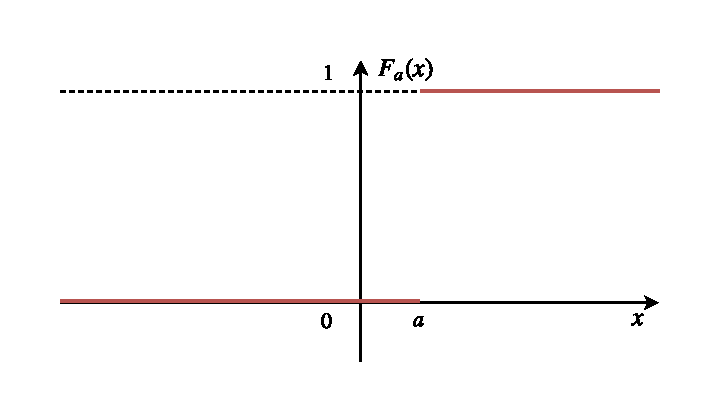
\includegraphics[width=\textwidth,height=\textheight,keepaspectratio]{fig/plot4-1.pdf}
	\end{center}
	\caption{$F_a(x)$.}
\end{figure}
	Рассмотрим
	\[
		1 \geqslant \Prob \left\{ \left| \frac{\sum\limits_{k = 1}^{n} \xi_k}{n} - a \leqslant \varepsilon \right| \right\} = \Prob \left\{ a - \varepsilon \leqslant \frac{\sum\limits_{k = 1}^{n} \xi_k}{n} \leqslant a + \varepsilon \right\}
	\]
	Сократим $[a - \varepsilon, a + \varepsilon]$
	\[
		\Prob \left\{ a - \frac{\varepsilon}{2} \leqslant \underbrace{\frac{\sum\limits_{k = 1}^{n} \xi_k}{n}}_{\eta_n} \leqslant a + \varepsilon \right\} =
	\]
	\[
		= F_{\eta_n} (a + \varepsilon) - F_{\eta_n} \left( a - \frac{\varepsilon}{2} \right) \underset{n \to \infty}{\rightarrow} F_a \left( a + \varepsilon \right) - F_a \left(a - \frac{\varepsilon}{2} \right) = 1
	\]
	\[
		\lim\limits_{n \to \infty} \Prob \left\{ | \eta_n - a | \leqslant \varepsilon \right\} = 1
	\]
\end{proof}
\begin{theorem}
	\textit{(Бернулли)} $\mu_n$, $B [n, p]$
	\[
		\forall \varepsilon > 0: \ \lim\limits_{n \to \infty} \Prob \left\{ \left| \frac{\mu_n}{n} - p \right| > \varepsilon \right\} = 0
	\]
\end{theorem}
Из теоремы Хинчина следует теорема Бернулли.
	\[
		\mu_n = \sum\limits_{k = 1}^{n} \xi_k,
	\]
	где $\xi_k$ --- число успеха в $k$-ом испытании Бернулли. \\
При большом числе испытаний относительная частота успеха стремится по вероятности к вероятности появления успеха. Число испытаний растёт, значит, относительная частота реже отличается от вероятности.
\begin{theorem}
	\textit{(Чебышёва)} $\{ \xi_n \}$ --- независимые случайные величины, пусть также имеющие дисперсию $\Variance_{\xi_k} = \sigma_k^2$
\[
	\forall k: \ \exists c: \sigma_k^2 \leqslant c
\]
значит, выполнен закон больших чисел. Пусть 
\[
	\eta_n = \frac{1}{n} \sum\limits_{k = 1}^{n} \xi_k, \ \MExpect_{\eta_n} = \frac{1}{n} \sum\limits_{k = 1}^{n} \MExpect_{\xi_k}
\]
\[
	\Variance_{\eta_n} = \frac{1}{n^2} \sum\limits_{k = 1}^{n} \sigma_k^2
\]
Рассмотрим:
\[
	\Prob \left\{ |\eta_n - \MExpect_{\eta_n} | > \varepsilon \right\} \leqslant \frac{\Variance_{\eta_n}}{\varepsilon^2} \leqslant \frac{c \cdot n}{n^2 \varepsilon^2} \underset{n \to \infty}{\rightarrow} 0
\]
\end{theorem}
\begin{theorem}
	\textit{(Маркова)}. Пусть $\xi_1, \ldots, \xi_n, \ldots$ --- случайные величины, имеющие дисперсию $\Variance_{\xi_k}$. Если
\[
	\frac{\Variance \left[ \sum\limits_{k = 1}^{n} \xi_k \right]}{n^2} \underset{n \to \infty}{\rightarrow} 0
\]
Тогда $\{ \xi_n \}$ подчиняется закону больших чисел.
\end{theorem}
\textbf{Усиленный закон больших чисел}. $\{ \xi_n \}$ --- последовательность случайных величин, имеющих математическое ожидание $\MExpect_{\xi_n}$
\[
	\frac{1}{n} \sum\limits_{k = 1}^{n} {\xi_k} \underset{n \to \infty}{\rightarrow} \frac{1}{n} \sum\limits_{k = 1}^{n} \MExpect_{\xi_k}
\]
\begin{theorem}
	\textit{(Колмогорова)}. $\{ \xi_n \}$ --- последовательность независимых случайных величин, имеющих дисперсию $\Variance_{\xi_n} = \sigma_n^2$. Если $\sum\limits_{n = 1}^{\infty} \frac{\sigma_n^2}{n^2}$ сходится, то $\{ \xi_n \}$ подчиняется усиленному закону больших чисел.
\end{theorem}

\section{Центральная предельная теорема}
Пусть $\xi_1, \ldots, \xi_n$ --- последовательность независимых случайных величин, каждая из которых имеет конечную дисперсию. Обозначим $\eta_n = \xi_1 + \ldots + \xi_n$. Говорят, что для последовательности выполнена центральная предельная теорема, если справедливо
\[
	\forall x \in \mathbb{R}^1: \ \lim\limits_{n \to \infty} \Prob \left\{ \frac{\eta_n - \MExpect_{\eta_n}}{\sqrt{\Variance_{\eta_n}}} \leqslant x \right\} = \frac{1}{\sqrt{2 \pi}} \int\limits_{-\infty}^{x} e^{- \frac{u^2}{2}} du = F_{N(0,1)} (x)
\]
Введём стандартизованную случайную величину, соответствующую $\eta_n$:
\[
	\widetilde{\eta}_n = \frac{\eta_n - \MExpect_{\eta_n}}{\sqrt{\Variance_{\eta_n}}}
\]
Итак,
\[
	F_{\widetilde{\eta}_n} (x) \underset{n \to \infty}{\rightarrow} F_{N(0, 1)} (x)
\]
\[
	\widetilde{\eta}_n \overset{d}{\rightarrow} \eta: \eta \sim N(0, 1)
\]
\begin{theorem}
	\textit{(Поля Леви)} Пусть $\xi_1, \ldots, \xi_n$ --- последовательность независимых, одинаково распределённых случайных величин, имеющих дисперсию $\Variance_{\xi_k} = \sigma^2 > 0$ и математическое ожидание $\MExpect_{\xi_k} = a$. Тогда выполнена ЦПТ для $\{ \xi_n \}_{n = 1, \ldots}$:
\[
	\forall x \in \mathbb{R}^1: \ \lim\limits_{n \to \infty} \Prob \left\{ \frac{\xi_1 + \ldots + \xi_n - na}{\sigma \sqrt{n}} \leqslant x \right\} = F_{N(0, 1)} (x)
\]
\end{theorem}
\begin{proof}
	Обозначим
	\[
		\sum\limits_{k = 1}^{n} \xi_k = \eta_n, \ \widetilde{\eta}_n = \frac{\xi_1 + \ldots + \xi_n - na}{\sigma \sqrt{n}} 
	\]
	Введём для каждой величины $\xi_k$ центрированную случайную величину
	\[
		\widetilde{\xi}_k = \xi_k - a
	\]
	Тогда
	\[
		\widetilde{\eta}_n = \frac{1}{\sigma \sqrt{n}} \sum\limits_{k = 1}^{n} \widetilde{\xi}_k
	\]
	\[
		\MExpect_{\widetilde{\xi}_k} = 0, \ \Variance_{\widetilde{\xi}_k} = \Variance_{\xi_k} = \MExpect_{\xi_k^2}
	\]
	Рассмотрим характеристическую функцию:
	\[
		\exists \MExpect_{|\xi|^n} \Rightarrow \phi_{\xi} (t) = \sum\limits_{k = 0}^{n} \frac{(it)^k}{k!} \MExpect_{\xi^k} + o(t^n)
	\]
	\[
		\forall t \in \mathbb{R}^1: \ \phi_{{\widetilde{\xi}_k}} (t) = 1 - \frac{t^2 \sigma^2}{2} + o(t^2)
	\]
	Перейдём к интересующей нас $\widetilde{\eta}_n$:
	\[
		\phi_{\widetilde{\eta}_n} (t) = \left[ \phi_{\widetilde{\xi}_k} \left( \frac{t}{\sigma \sqrt{n}} \right) \right]^n = \left[ 1 - \frac{t^2}{n \cdot 2} + o \left( \frac{t^2}{n} \right) \right]^n \underset{n \to \infty}{\rightarrow} e^{- \frac{t^2}{2}}
	\]
	Известно, что $\phi_{N(0, 1)} = e^{- \frac{t^2}{2}}$
	Итак,
	\[
		\forall t \in \mathbb{R}^1: \ \phi_{\widetilde{\eta}_n} (t) \underset{n \to \infty}{\rightarrow} \phi_{N(0, 1)}
	\]
	Значит, по теореме непрерывности:
	\[
		\forall x \in \mathbb{R}^1: \ F_{\widetilde{\eta}_n} \underset{n \to \infty}{\rightarrow} F_{N(0, 1)} (x)
	\]
	Значит, ЦПТ выполнена для $\{ \xi_n \}_{n = 1, \ldots}$
\end{proof}
\begin{theorem}
	\textit{(Муавра-Лапласа)} Распределения числа успехов в схеме испытаний Бернулли при фиксированной вероятности появления успеха $p$ не близкой к 1 и 0 при стремлении числа испытаний к бесконечности имеет место соотношение:
\[
	B[n, p], \ \mu_n, \ 0 < p < 1, q = 1 - p
\]
где $p$ фиксировано
\[
	\forall x \in \mathbb{R}^1: \ \lim\limits_{n \to \infty} \Prob \left\{ \frac{\mu_n - n \cdot p}{\sqrt{n \cdot p \cdot q}} \leqslant x \right\} = F_{N(0, 1)} (x)
\]
\end{theorem}
\begin{proof}
	Из теоремы Поля Леви:
	\[
		\mu_n = \sum\limits_{k = 1}^{n} \xi_k,
	\]
	где $\xi_k$ --- число появления «успеха» в $k$-ом испытании.
	\[
		\Variance_{\xi_k} = pq
	\]
	Для $\{ \xi_n \}_{n = 1, \ldots}$ --- бернуллиевских выполнена ЦПТ.
\end{proof}
\[
	\mu_n \sim N(np, \sqrt{npq})
\]
Пусть $\xi_1, \ldots, \xi_n$ --- набор независимых случайных величин, имеющих дисперсию $\Variance_{\xi_k}$, при этом $\sum\limits_{k = 1}^{n} \Variance_{\xi_k} > 0$. Рассмотрим $\xi_k$.
\[
	\MExpect_{\xi_k} = a_k, \ \Variance_{\xi_k} = \sigma_k^2, \ F_k(x) \text{ --- функция распределения $F_k(x)$}
\]
\[
	\sum\limits_{k = 1}^{n} \sigma_k^2 = B_n^2, \ \lambda_n = max \frac{\sigma_k^2}{B_n^2}, \ B_n = \sqrt{B_n^2}
\]
Пусть $\varepsilon > 0$, введём
\[ 
	\mathcal{L}_n(\varepsilon) = \frac{1}{B^2_n} \sum\limits_{k = 1}^{n} \int\limits_{\omega} (x - a_k)^2 dF_k (x)
\] 
где $\omega = \{ x: |x - a_k| \geqslant \varepsilon \cdot B_n \}$. \\
Будем говорить, что выполнено условие Линдеберга, если
\[
	\forall \varepsilon > 0: \ \lim\limits_{n \to \infty} \mathcal{L}_n (\varepsilon) = 0
\]
\begin{theorem}
	\textit{(Линдеберга)}. Пусть для $\xi_1, \ldots, \xi_n, \ldots$ --- набора независимых случайных величин, имеющих конечную дисперсию $\Variance_{\xi_k}$, выполнено условие Линдеберга. Тогда
\begin{enumerate}
	\item $\{ \xi_n \}_{n = 1, \ldots}$ подчиняется ЦПТ.
	\item $\lambda_n \underset{n \to \infty}{\rightarrow} 0$
\end{enumerate}
И также из (1, 2) следует выполнимость условия Линдеберга. \\
$\lambda_n \underset{n \to \infty}{\rightarrow} 0$ означает, что каждое слагаемое в $\eta_n = \sum\limits_{k = 1}^{n} \xi_k$ пренебрежимо мало по сравнению с $\eta_n$
\end{theorem}
\begin{conclusion}
\textit{Теорема Поля Леви.}  $\{ \xi_n \}$ --- последовательность одинаково распределённых случайных величин. Рассмотрим $\mathcal{L}_n (\varepsilon)$ для фиксированного $\varepsilon > 0$:
\[
	\mathcal{L}_n (\varepsilon) = \frac{1}{\sigma^2 n} \sum\limits_{k = 1}^{n} \int\limits_{\omega} (x - a)^2 d F(x) =
\]
где $\omega = \{ x: |x - a_k| \geqslant \varepsilon \cdot \sigma \sqrt{n} \}$
\[
	\frac{1}{\sigma^2} \int\limits_{\omega} (x - a)^2 dF(x) \rightarrow 0 \Rightarrow \text{ $\{ \xi_n \}$ подчиняется ЦПТ.}
\]
\end{conclusion}
\begin{conclusion}
\textit{Теорема Ляпунова.} Пусть $\{ \xi_n \}_{n = 1, \ldots}$ --- последовательность независимых случайных величин, имеющих дисперсию $\Variance_{\xi_k}$
\[
	\forall k = 1, 2, \ldots : \ \exists \delta > 0: \exists \underbrace{\MExpect \left[ |x - a_k|^{2 + \delta}\right]}_{\alpha_k} < \infty
\]
Составим дробь Ляпунова:
\[
	L_n = \frac{\sum\limits_{k = 1}^{n} \alpha_k}{B_n^{2 + \delta}}
\]
Тогда 
\[
	L_n \underset{n \to \infty}{\rightarrow} 0 \Rightarrow \text{ для $\{ \xi_n \}_{n = 1, \ldots}$ выполняется ЦПТ.}
\]
\end{conclusion}
\begin{proof}
	Пусть для любого $\varepsilon > 0$
	\[
		\mathcal{L}_n (\varepsilon) \leqslant \frac{1}{\varepsilon^{\delta} \cdot B_n^{2 + \delta}} \cdot \sum\limits_{k = 1}^{n} \int\limits_{\omega} |x - a_k|^{2 + \delta} dF_k(x) \leqslant \frac{\sum\limits_{k = 1}^{n} \alpha_k}{\varepsilon^{\delta} \cdot B_n^{2 + \delta}} \underset{n \to \infty}{\rightarrow} 0
	\]
	где $\omega = \{ x: |x - a_k| \geqslant \varepsilon \cdot B_n \}$.
\end{proof}
\begin{theorem}
	\textit{(Стеклова)}. Пусть $\{ \xi_n \}_{n = 1, \ldots}$ --- последовательность независимых равномерно ограниченных случайных величин, имеющих дисперсию $\Variance_{\xi_k}$, при этом 
\[
	\forall k: \ |\xi_k| \leqslant K, \ K = const
\]
Тогда
\[
	B_n \underset{n \to \infty}{\rightarrow} + \infty \Rightarrow \{ \xi_n \}_{n = 1, \ldots} \text{ подчиняется ЦПТ.}
\]
\end{theorem}
\begin{proof}
	$\varepsilon > 0$:
	\[
		\int\limits_{S} (x - a_k)^2 dF_k (x) = \MExpect [(\xi_k - a_k)^2 \cdot I_A (\omega)]
	\]
	где $S = \{ x: \ |x - a_k| \geqslant \varepsilon B_n \}$, $A = \{ |\xi_k - a_k | \geqslant \varepsilon \cdot B_n \}$.
	\[
		\MExpect [(\xi_k - a_k)^2 \cdot I_A (\omega)] \leqslant (2K)^2 \Prob (S) \overset{\text{нер-во Чебышёва}}{\leqslant} (2K)^2 \frac{\sigma_k^2}{\varepsilon^2 \cdot B_n^2}
	\]
	Теперь оценим $\mathcal{L}_n(\varepsilon)$
	\[
		\mathcal{L}_n (\varepsilon) \leqslant \frac{(2K)^2}{\varepsilon^2 B_n^2} \underset{n \to \infty}{\rightarrow} 0
	\]
\end{proof}
Вообще класс предельных распределений сумм квадратов случайных величин не исчерпывается нормальным. \\

Закон называется безгранично-делимым, если его характеристическую функцию можно представить как другую функцию в $n$-ой степени:
\[
	\forall n : \ \phi(t) = \left[ \widetilde{\phi} (t) \right]^n
\]
Нормальный закон также можно представить таким образом (и $\Gamma$-распределение, и распределение Пуассона, и др.) \\

Если на величину какого-то признака влияет много независимых случайных факторов, и влияние каждого из них невелико, однако суммарное ощутимо, то закон распределения этой величины можно считать нормальным.



